\documentclass{standalone}
\usepackage{tikz}
\usetikzlibrary{patterns, positioning}

\begin{document}
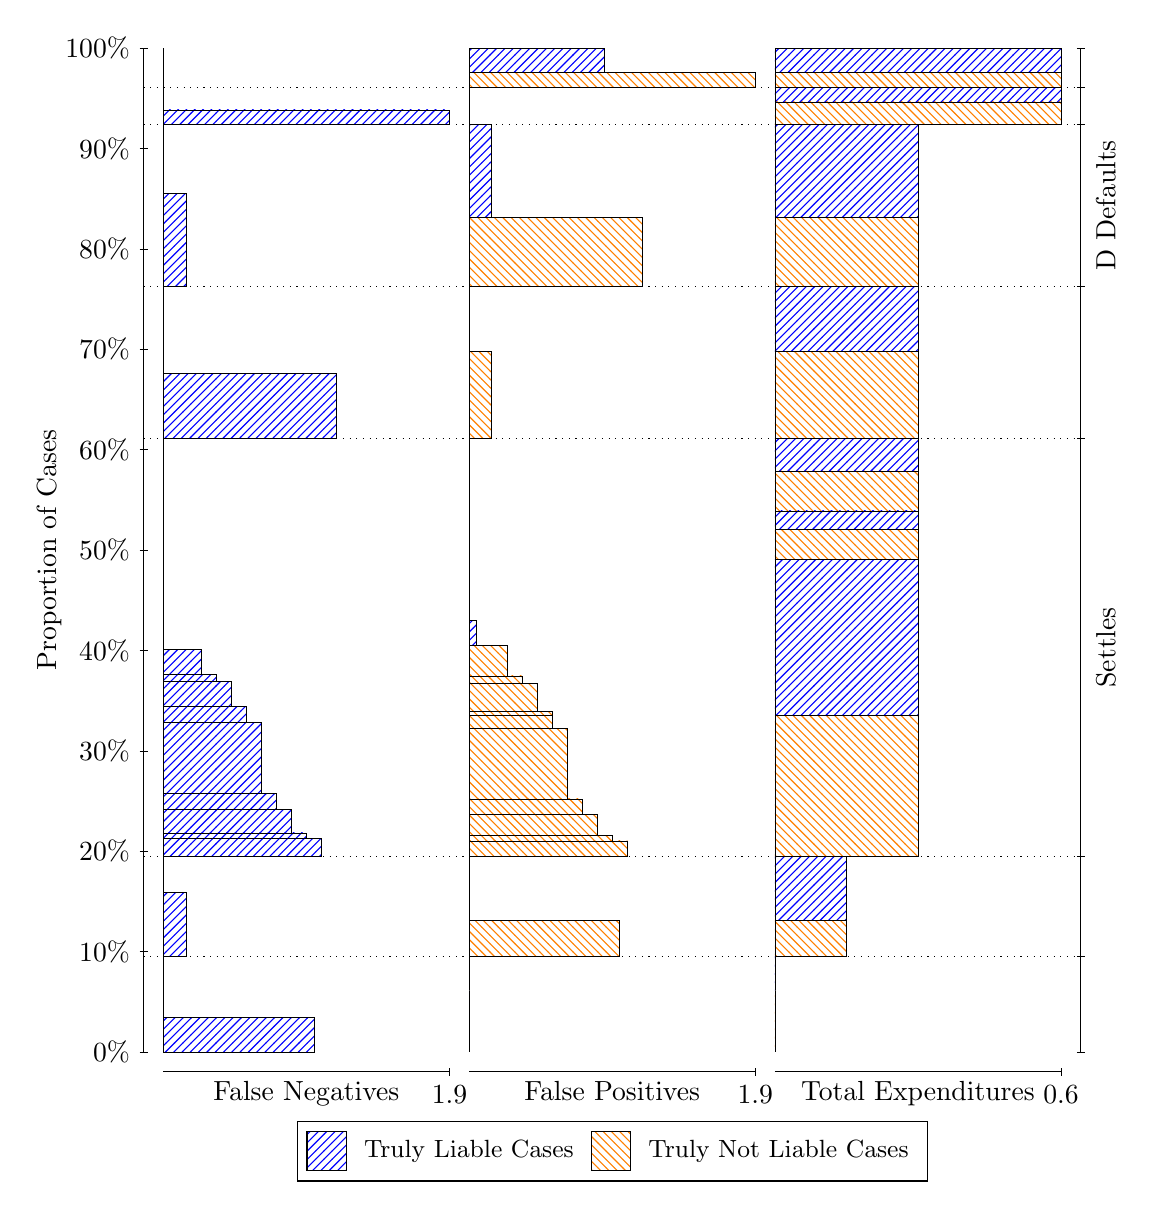
\begin{tikzpicture}
\draw[black, very thin] (1.5,1.75) -- (1.5,14.5);
\node[rotate=90, anchor=center] at (0.3, 8.125) {Proportion of Cases};
\draw[black, very thin] (1.45,1.75) -- (1.55,1.75);
\node[anchor=east] at (1.45, 1.75) {0\%};
\draw[black, very thin] (1.45,3.025) -- (1.55,3.025);
\node[anchor=east] at (1.45, 3.025) {10\%};
\draw[black, very thin] (1.45,4.3) -- (1.55,4.3);
\node[anchor=east] at (1.45, 4.3) {20\%};
\draw[black, very thin] (1.45,5.575) -- (1.55,5.575);
\node[anchor=east] at (1.45, 5.575) {30\%};
\draw[black, very thin] (1.45,6.85) -- (1.55,6.85);
\node[anchor=east] at (1.45, 6.85) {40\%};
\draw[black, very thin] (1.45,8.125) -- (1.55,8.125);
\node[anchor=east] at (1.45, 8.125) {50\%};
\draw[black, very thin] (1.45,9.4) -- (1.55,9.4);
\node[anchor=east] at (1.45, 9.4) {60\%};
\draw[black, very thin] (1.45,10.675) -- (1.55,10.675);
\node[anchor=east] at (1.45, 10.675) {70\%};
\draw[black, very thin] (1.45,11.95) -- (1.55,11.95);
\node[anchor=east] at (1.45, 11.95) {80\%};
\draw[black, very thin] (1.45,13.225) -- (1.55,13.225);
\node[anchor=east] at (1.45, 13.225) {90\%};
\draw[black, very thin] (1.45,14.5) -- (1.55,14.5);
\node[anchor=east] at (1.45, 14.5) {100\%};

\draw[black, very thin] (13.4,1.75) -- (13.4,14.5);
\draw[black, very thin] (13.35,1.75) -- (13.45,1.75);
\node[anchor=west] at (13.35, 1.75) {};
\draw[black, very thin] (13.35,2.9674) -- (13.45,2.9674);
\node[anchor=west] at (13.35, 2.9674) {};
\draw[black, very thin] (13.35,4.235) -- (13.45,4.235);
\node[anchor=west] at (13.35, 4.235) {};
\draw[black, very thin] (13.35,9.5421) -- (13.45,9.5421);
\node[anchor=west] at (13.35, 9.5421) {};
\draw[black, very thin] (13.35,11.472) -- (13.45,11.472);
\node[anchor=west] at (13.35, 11.472) {};
\draw[black, very thin] (13.35,13.527) -- (13.45,13.527);
\node[anchor=west] at (13.35, 13.527) {};
\draw[black, very thin] (13.35,14.003) -- (13.45,14.003);
\node[anchor=west] at (13.35, 14.003) {};
\draw[black, very thin] (13.35,14.5) -- (13.45,14.5);
\node[anchor=west] at (13.35, 14.5) {};

\draw[black, very thin, pattern color=blue, pattern=north east lines] (1.75,1.75) rectangle (3.6623,2.1873);
\draw[black, very thin, pattern color=orange, pattern=north west lines] (1.75,2.1873) rectangle (1.75,2.9674);
\draw[black, very thin, pattern color=blue, pattern=north east lines] (1.75,2.9674) rectangle (2.0368,3.7781);
\draw[black, very thin, pattern color=orange, pattern=north west lines] (1.75,3.7781) rectangle (1.75,4.235);
\draw[black, very thin, pattern color=blue, pattern=north east lines] (1.75,4.235) rectangle (3.7579,4.467);
\draw[black, very thin, pattern color=blue, pattern=north east lines] (1.75,4.467) rectangle (3.5667,4.5329);
\draw[black, very thin, pattern color=blue, pattern=north east lines] (1.75,4.5329) rectangle (3.3754,4.8294);
\draw[black, very thin, pattern color=blue, pattern=north east lines] (1.75,4.8294) rectangle (3.1842,5.0293);
\draw[black, very thin, pattern color=blue, pattern=north east lines] (1.75,5.0293) rectangle (2.993,5.9347);
\draw[black, very thin, pattern color=blue, pattern=north east lines] (1.75,5.9347) rectangle (2.8018,6.1431);
\draw[black, very thin, pattern color=blue, pattern=north east lines] (1.75,6.1431) rectangle (2.6105,6.4574);
\draw[black, very thin, pattern color=blue, pattern=north east lines] (1.75,6.4574) rectangle (2.4193,6.5424);
\draw[black, very thin, pattern color=blue, pattern=north east lines] (1.75,6.5424) rectangle (2.2281,6.8673);
\draw[black, very thin, pattern color=orange, pattern=north west lines] (1.75,6.8673) rectangle (1.75,9.5421);
\draw[black, very thin, pattern color=blue, pattern=north east lines] (1.75,9.5421) rectangle (3.9491,10.365);
\draw[black, very thin, pattern color=orange, pattern=north west lines] (1.75,10.365) rectangle (1.75,11.472);
\draw[black, very thin, pattern color=blue, pattern=north east lines] (1.75,11.472) rectangle (2.0368,12.653);
\draw[black, very thin, pattern color=orange, pattern=north west lines] (1.75,12.653) rectangle (1.75,13.527);
\draw[black, very thin, pattern color=blue, pattern=north east lines] (1.75,13.527) rectangle (5.3833,13.713);
\draw[black, very thin, pattern color=orange, pattern=north west lines] (1.75,13.713) rectangle (1.75,14.003);
\draw[black, very thin, pattern color=orange, pattern=north west lines] (1.75,14.003) rectangle (1.75,14.195);
\draw[black, very thin, pattern color=blue, pattern=north east lines] (1.75,14.195) rectangle (1.75,14.5);
\draw[black, very thin, pattern color=orange, pattern=north west lines] (5.6333,1.75) rectangle (5.6333,2.5301);
\draw[black, very thin, pattern color=blue, pattern=north east lines] (5.6333,2.5301) rectangle (5.6333,2.9674);
\draw[black, very thin, pattern color=orange, pattern=north west lines] (5.6333,2.9674) rectangle (7.5456,3.4243);
\draw[black, very thin, pattern color=blue, pattern=north east lines] (5.6333,3.4243) rectangle (5.6333,4.235);
\draw[black, very thin, pattern color=orange, pattern=north west lines] (5.6333,4.235) rectangle (7.6412,4.4303);
\draw[black, very thin, pattern color=orange, pattern=north west lines] (5.6333,4.4303) rectangle (7.45,4.4958);
\draw[black, very thin, pattern color=orange, pattern=north west lines] (5.6333,4.4958) rectangle (7.2588,4.7665);
\draw[black, very thin, pattern color=orange, pattern=north west lines] (5.6333,4.7665) rectangle (7.0675,4.9632);
\draw[black, very thin, pattern color=orange, pattern=north west lines] (5.6333,4.9632) rectangle (6.8763,5.86);
\draw[black, very thin, pattern color=orange, pattern=north west lines] (5.6333,5.86) rectangle (6.6851,6.0202);
\draw[black, very thin, pattern color=orange, pattern=north west lines] (5.6333,6.0202) rectangle (6.6851,6.0799);
\draw[black, very thin, pattern color=orange, pattern=north west lines] (5.6333,6.0799) rectangle (6.4939,6.4333);
\draw[black, very thin, pattern color=orange, pattern=north west lines] (5.6333,6.4333) rectangle (6.3026,6.5263);
\draw[black, very thin, pattern color=orange, pattern=north west lines] (5.6333,6.5263) rectangle (6.1114,6.9098);
\draw[black, very thin, pattern color=blue, pattern=north east lines] (5.6333,6.9098) rectangle (5.7289,7.2347);
\draw[black, very thin, pattern color=blue, pattern=north east lines] (5.6333,7.2347) rectangle (5.6333,9.5421);
\draw[black, very thin, pattern color=orange, pattern=north west lines] (5.6333,9.5421) rectangle (5.9202,10.649);
\draw[black, very thin, pattern color=blue, pattern=north east lines] (5.6333,10.649) rectangle (5.6333,11.472);
\draw[black, very thin, pattern color=orange, pattern=north west lines] (5.6333,11.472) rectangle (7.8325,12.347);
\draw[black, very thin, pattern color=blue, pattern=north east lines] (5.6333,12.347) rectangle (5.9202,13.527);
\draw[black, very thin, pattern color=orange, pattern=north west lines] (5.6333,13.527) rectangle (5.6333,13.817);
\draw[black, very thin, pattern color=blue, pattern=north east lines] (5.6333,13.817) rectangle (5.6333,14.003);
\draw[black, very thin, pattern color=orange, pattern=north west lines] (5.6333,14.003) rectangle (9.2667,14.195);
\draw[black, very thin, pattern color=blue, pattern=north east lines] (5.6333,14.195) rectangle (7.3544,14.5);
\draw[black, very thin, pattern color=orange, pattern=north west lines] (9.5167,1.75) rectangle (9.5167,2.5301);
\draw[black, very thin, pattern color=blue, pattern=north east lines] (9.5167,2.5301) rectangle (9.5167,2.9674);
\draw[black, very thin, pattern color=orange, pattern=north west lines] (9.5167,2.9674) rectangle (10.425,3.4243);
\draw[black, very thin, pattern color=blue, pattern=north east lines] (9.5167,3.4243) rectangle (10.425,4.235);
\draw[black, very thin, pattern color=orange, pattern=north west lines] (9.5167,4.235) rectangle (11.333,6.0202);
\draw[black, very thin, pattern color=blue, pattern=north east lines] (9.5167,6.0202) rectangle (11.333,8.0071);
\draw[black, very thin, pattern color=orange, pattern=north west lines] (9.5167,8.0071) rectangle (11.333,8.3906);
\draw[black, very thin, pattern color=blue, pattern=north east lines] (9.5167,8.3906) rectangle (11.333,8.6225);
\draw[black, very thin, pattern color=orange, pattern=north west lines] (9.5167,8.6225) rectangle (11.333,9.1286);
\draw[black, very thin, pattern color=blue, pattern=north east lines] (9.5167,9.1286) rectangle (11.333,9.5421);
\draw[black, very thin, pattern color=orange, pattern=north west lines] (9.5167,9.5421) rectangle (11.333,10.649);
\draw[black, very thin, pattern color=blue, pattern=north east lines] (9.5167,10.649) rectangle (11.333,11.472);
\draw[black, very thin, pattern color=orange, pattern=north west lines] (9.5167,11.472) rectangle (11.333,12.347);
\draw[black, very thin, pattern color=blue, pattern=north east lines] (9.5167,12.347) rectangle (11.333,13.527);
\draw[black, very thin, pattern color=orange, pattern=north west lines] (9.5167,13.527) rectangle (13.15,13.817);
\draw[black, very thin, pattern color=blue, pattern=north east lines] (9.5167,13.817) rectangle (13.15,14.003);
\draw[black, very thin, pattern color=orange, pattern=north west lines] (9.5167,14.003) rectangle (13.15,14.195);
\draw[black, very thin, pattern color=blue, pattern=north east lines] (9.5167,14.195) rectangle (13.15,14.5);
\draw[black, dotted] (1.5,2.9674) -- (13.4,2.9674);
\draw[black, dotted] (1.5,4.235) -- (13.4,4.235);
\draw[black, dotted] (1.5,9.5421) -- (13.4,9.5421);
\draw[black, dotted] (1.5,11.472) -- (13.4,11.472);
\draw[black, dotted] (1.5,13.527) -- (13.4,13.527);
\draw[black, dotted] (1.5,14.003) -- (13.4,14.003);
\draw[black, very thin] (1.75,1.5) -- (5.3833,1.5);
\node[anchor=north] at (3.5667, 1.5) {False Negatives};
\draw[black, very thin] (5.3833,1.45) -- (5.3833,1.55);
\node[anchor=north] at (5.3833, 1.45) {1.9};

\draw[black, very thin] (5.6333,1.5) -- (9.2667,1.5);
\node[anchor=north] at (7.45, 1.5) {False Positives};
\draw[black, very thin] (9.2667,1.45) -- (9.2667,1.55);
\node[anchor=north] at (9.2667, 1.45) {1.9};

\draw[black, very thin] (9.5167,1.5) -- (13.15,1.5);
\node[anchor=north] at (11.333, 1.5) {Total Expenditures};
\draw[black, very thin] (13.15,1.45) -- (13.15,1.55);
\node[anchor=north] at (13.15, 1.45) {0.6};



\node[black, centered, rotate=90] at (13.72, 6.8885) {Settles};

\node[black, centered, rotate=90] at (13.72, 12.5) {D Defaults};



\draw (7.449999999999999,1.5) node[draw=none] (baseCoordinate) {};
\begin{scope}[align=center]
        \matrix[scale=0.5, draw=black, below=0.5cm of baseCoordinate, nodes={draw}, column sep=0.1cm]{
            \node[rectangle, draw, minimum width=0.5cm, minimum height=0.5cm, pattern=north east lines, pattern color=blue] {}; &
            \node[draw=none, font=\small] (B) {Truly Liable Cases}; &
            \node[rectangle, draw, minimum width=0.5cm, minimum height=0.5cm, pattern=north west lines, pattern color=orange] {}; &
            \node[draw=none, font=\small] (B) {Truly Not Liable Cases}; \\
            };
\end{scope}

\end{tikzpicture}
\end{document}